\chapter{Fenómenos Ondulatorios}% \label{lbl-fenomenos}
% Refelexion
\section{Reflexión}% \label{lbl-reflexion}
Es el cambio de dirección que experimenta un onda cuando choca contra una superficie y regresa al medio del cual provenie. Las superficies planas y duras reflejan más. Esto ocurre con diversas ondas como luz, sonido y las ondas en la superficie del agua.

\begin{figure}[H]
  \centering
  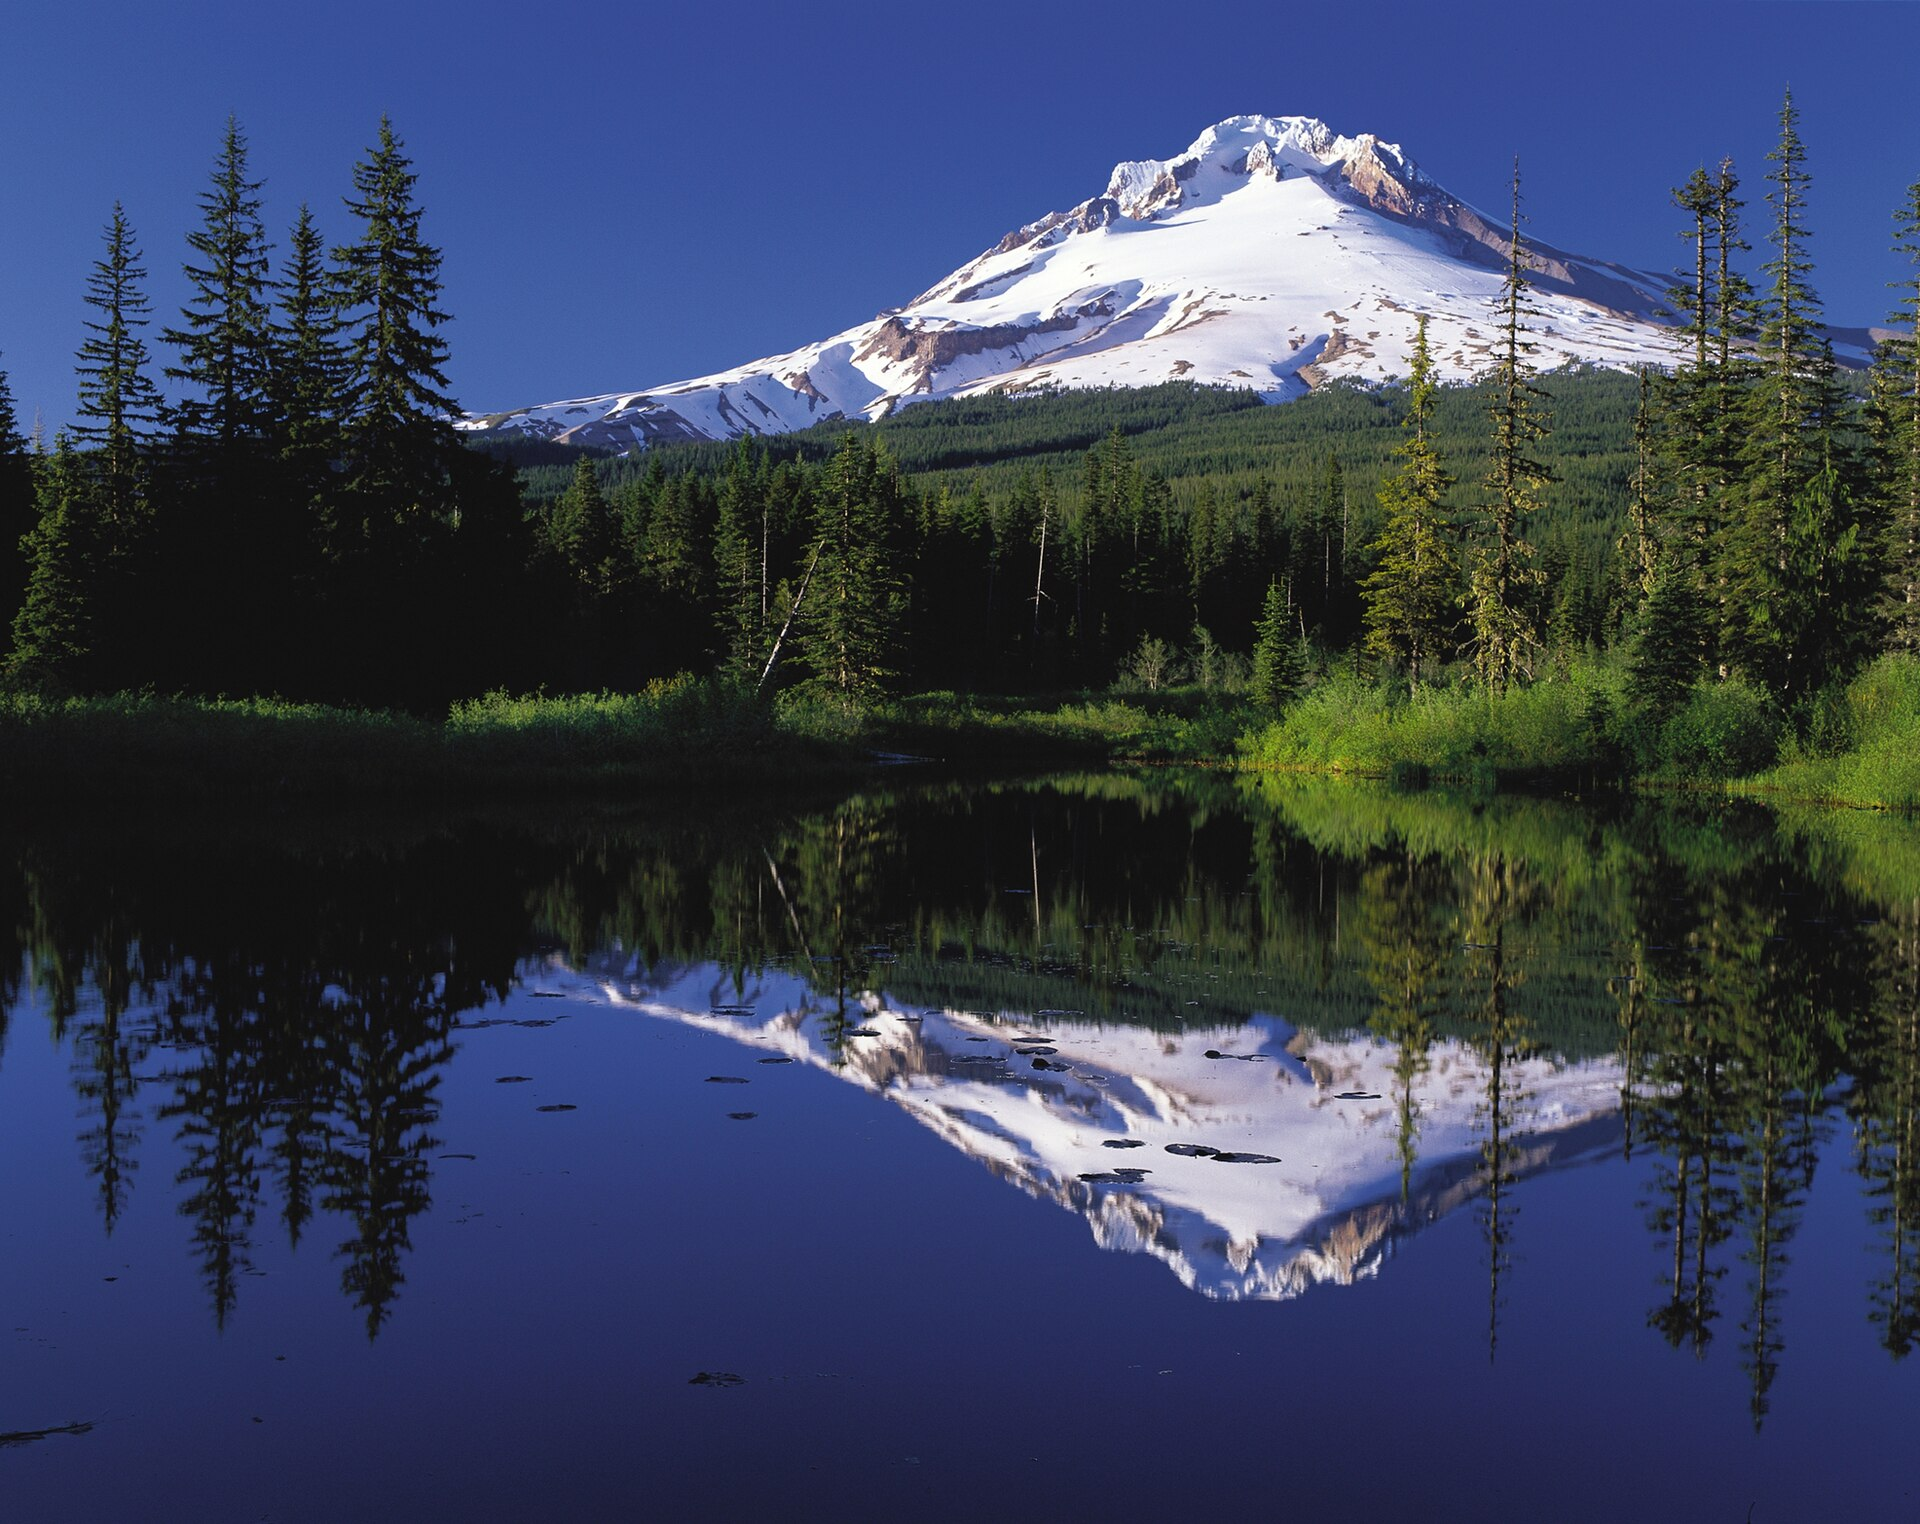
\includegraphics[scale=0.15]{imagenes/reflexion_monte.png}
  \caption{Reflexión en el agua\cite{wikireflexion}}
\end{figure}

El \textbf{eco} es un ejemplo de este fenómeno. Cuando una onda sonora choca contra una superficie, parte de la energía de la onda se refleja. Esto se percibe como un sonido distinto al original, debido a la separación temporal entre la onda emitida y reflejada. También se puede mencionar la \textbf{reverberación}, en este caso en un reflejo continuo de la onda de sonido.

La luz es otro caso preponderante. Toda la luz percibida por el ojo humano es el resultado de un rebote de las ondas de luz al chocar con multitud de superficies. Cuando el ojo no recibe ondas de luz, como en lugares oscuros o en la noche, entonces percibe oscuridad. La luz de estrellas lejanas llega constantemente hasta el planeta tierra, aunque durante el día es opacada por la luz solar emitida por el sol ubicado en el centro del sistema solar donde se encuentra la tierra.

\subsection{Ley de Reflexión}
Establece que el ángulo de incidencia de un rayo en una superficie es igual al ángulo de reflexión, ambos medidos con respecto a la normal de la superficie.

\begin{figure}[H]
  \centering
  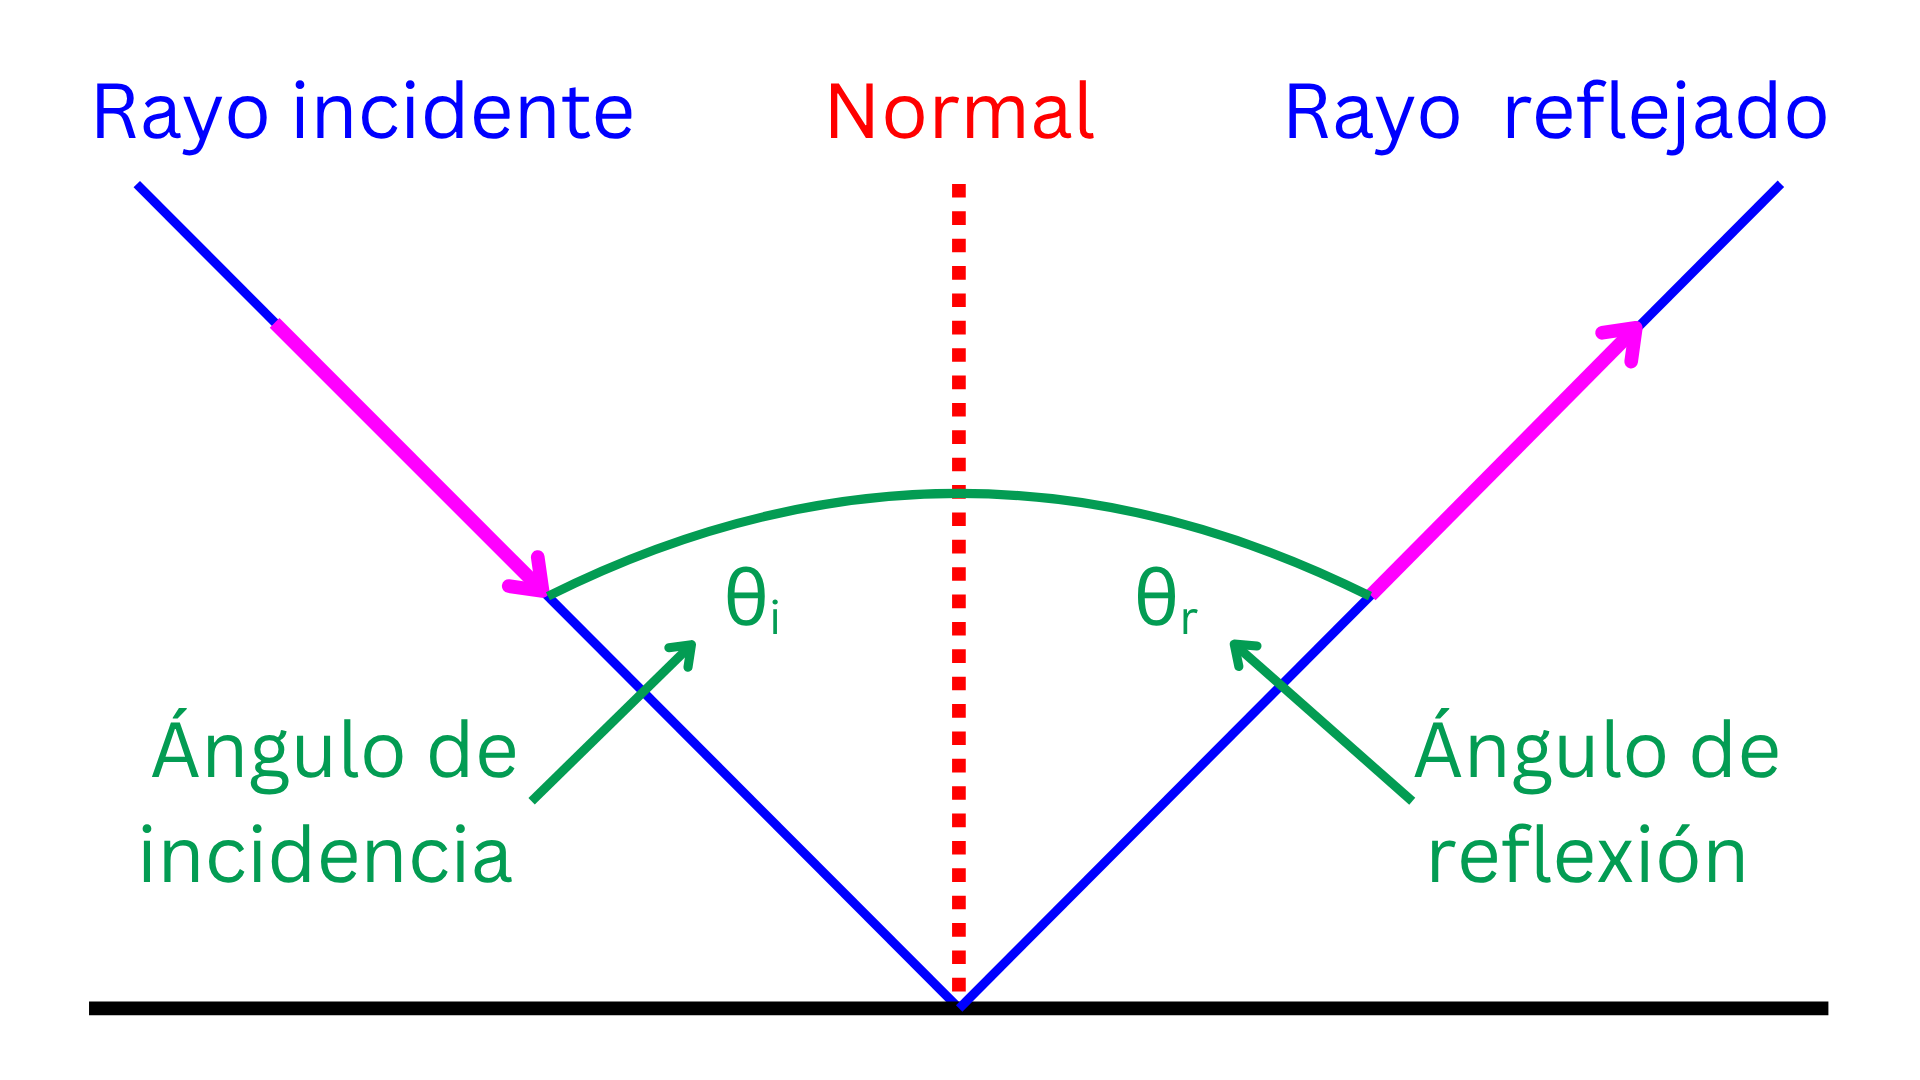
\includegraphics[scale=0.2]{imagenes/ley_reflexion.png}
  \caption{Ley de reflexión}
\end{figure}

Elementos:

\begin{itemize}
  \item \textbf{Rayo incidente:} Onda que entra o impacta con la superficie.
  \item \textbf{Rayo reflejado:} Onda que sale o rebota de la superficie.
  \item \textbf{Normal:} Linea imaginaria perpendicular a la superficie en el punto donde el rayo incide.
  \item \textbf{Ángulo de incidencia $(\theta_i)$:} Ángulo formado entre el rayo incidente y la normal.
  \item \textbf{Ángulo de reflexión $(\theta_r)$:} Ángulo formado entre el rayo reflejado y la normal.
\end{itemize}

Considerando un ángulo de incidencia $\theta_i$ y un ángulo de reflexión $\theta_r$, la ley se expresa de la siguiente forma:

\begin{listequbox}
  {\theta_i = \theta_r}{equleyrfl}{Ley de reflexión}
\end{listequbox}

\subsection{Reflexión Especular}
Los rayos reflejados se mantienen en un ángulo igual al ángulo de incidencia, produciendo una imagen clara y definida. Ocurre principalmente en superficies lisas y pulidas como espejos, agua en equilibrio y metales pulidos.

\begin{figure}[H]
  \centering
  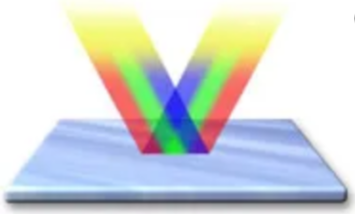
\includegraphics[scale=0.5]{imagenes/reflexion_especular.png}
  \caption{Reflexión especular\cite{sncrflspcdif}}
\end{figure}

\subsection{Reflexión Difusa}
Los rayos se dispersan en múltiples direcciones al incidir sobre una superficie rugosa o irregular. Esto forma imágenes que no son claras. La mayoría de los objetos en el ambiente reflejan la luz de forma difusa como la ropa, las paredes, el suelo, los árboles y otros.

\begin{figure}[H]
  \centering
  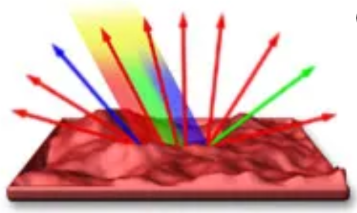
\includegraphics[scale=0.5]{imagenes/reflexion_difusa.png}
  \caption{Reflexión especular\cite{sncrflspcdif}}
\end{figure}

% Refraccion
\section{Refracción}
Cambio de dirección que experimenta una onda al pasar de un medio a otro con diferenta velocidad de propagación. Esto ocurre porque la onda cambia de velocidad al entrar en el nuevo medio, lo que provoca que se desvíe de su trayectoria original.

Cada medio, debido a sus propiedades físicas, tiene una velocidad de propagación diferente. Cuando las ondas interactuan con cada medio, su trayectoria está condicionada por la velocidad con la que se mueve dentro de se medio\cite{sncrfrlight}.

\begin{figure}
  \centering
  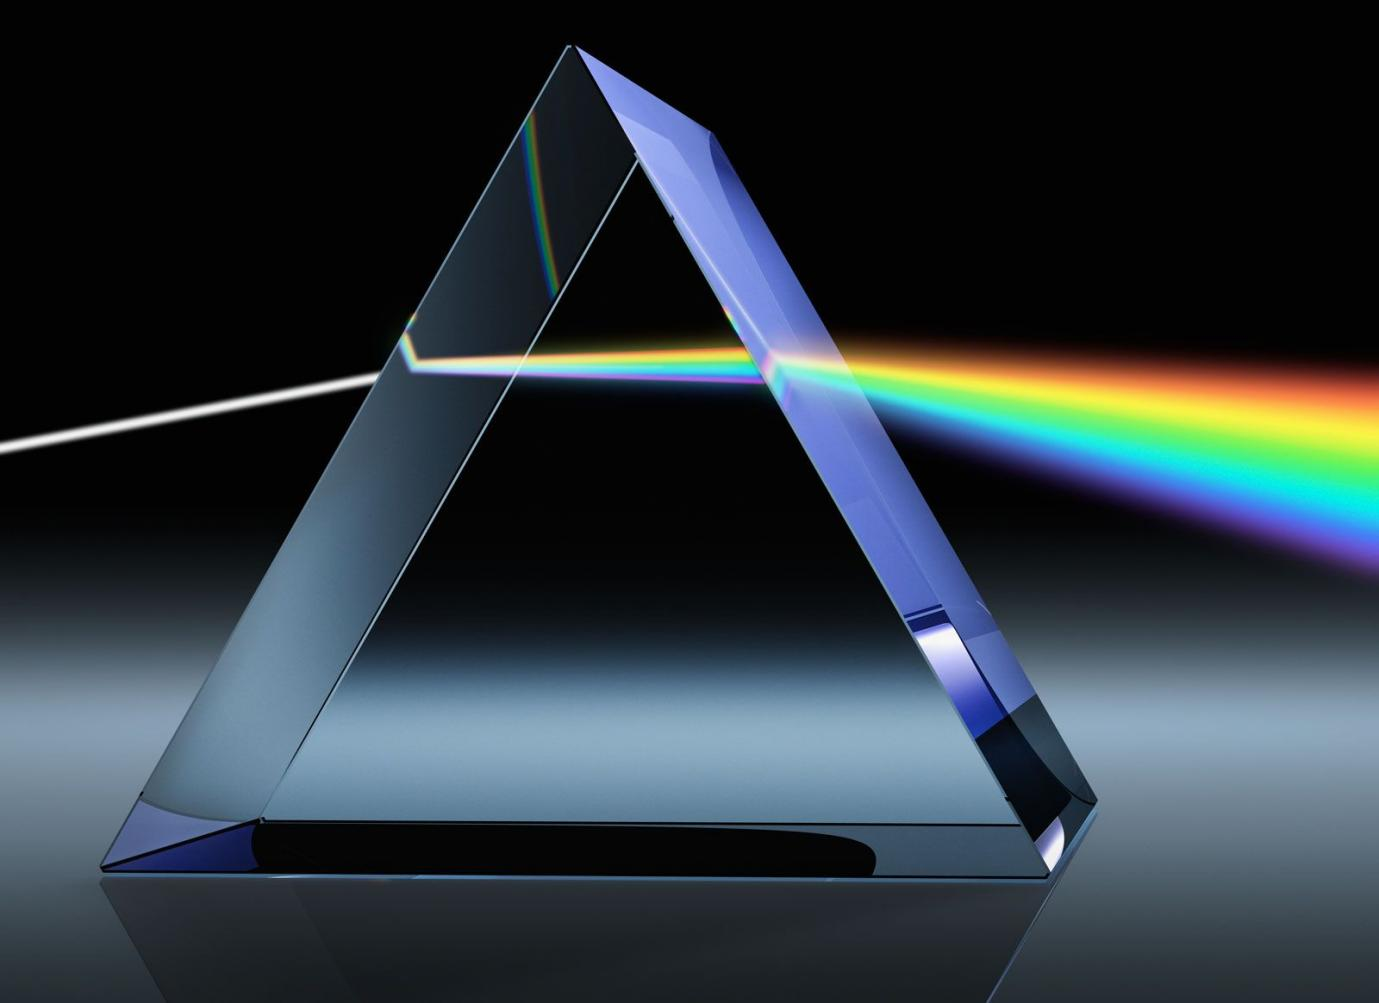
\includegraphics[scale=0.5]{imagenes/prisma.png}
  \caption{Refracción en un prisma\cite{cstmglassprism}}
\end{figure}

La refracción ocurre todo el tiempo. Se usa para enfocar la luz y crear imagenes claras mediante lentes de gafas, cámaras telescopios, microscopios y otros. Los arcoiris ocurren cuando la luz se refracta en las gotas de lluvia. Los objetos en el agua parecen estar doblados por efecto de la refracción.

Un gran ejemplos son los prismas hechos cristal o vidrio. La luz blanca, que es la combinación de todos los colores, al pasar a través del prisma se descompone en un espectro de colores como un arcoiris. Esto se debe a la distinta longitud de onda de los colores en el rango de luz visible.

\subsection{Ley de Snell}
\begin{figure}[H]
  \centering
  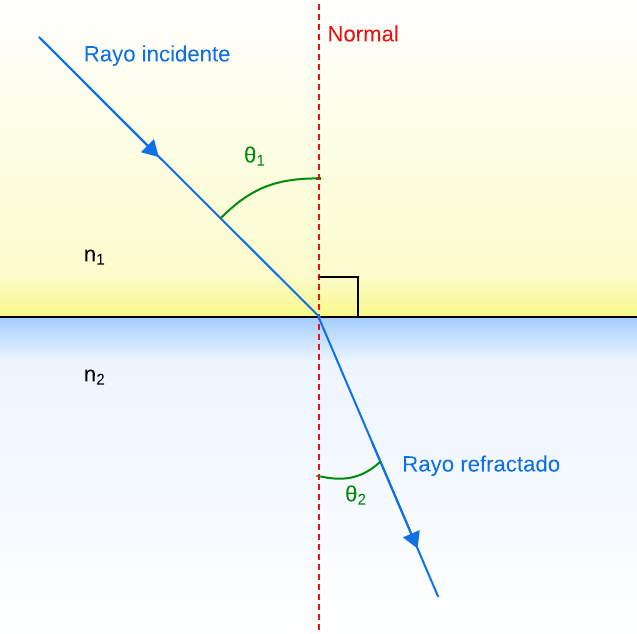
\includegraphics{imagenes/ley_snell.png}
  \caption{Ley de Snell}
\end{figure}

La formulación matemática es la siguiente:

\begin{listequbox}
  {n_1 \sin(\theta_1)=n_2 \sin(\theta_2)}{equleysnell}{Ley de Snell}
\end{listequbox}

Esta ley también es conocida como \textbf{Ley de refracción}.

Elementos:

\begin{itemize}
  \item \textbf{Rayo incidente:} Onda que viene de un primer medio y pasa a un segundo medio.
  \item \textbf{Rayo refractado:} Onda dentro de un segundo medio.
  \item \textbf{Normal:} Linea imaginaria perpendicular a la linea de separación entre ambos medios, en el punto donde el rayo incide.
  \item \textbf{Ángulo de incidencia $(\theta_1)$:} Ángulo formado entre el rayo incidente y la normal.
  \item \textbf{Ángulo de refracción $(\theta_2)$:} Ángulo formado entre el rayo refractado y la normal.
  \item \textbf{Índice de refracción 1 $(n_1)$:} Índice de refracción en el primer medio.
  \item \textbf{Índice de refracción 2 $(n_2)$:} Índice de refracción en el segundo medio.
\end{itemize}

El \textbf{índice de refracción}, representado por la letra $n$ minúscula, es una medida de como la luz se refracta al pasar de un medio a otro. Un índice más alto indica la onda viaja más lento, y en sentido contrario un índice más bajo indica que la onda viaja más rápido. Se calcula dividiendo la velocidad de la luz en el vacío $(c)$, ecuación \ref{equvelluz}, entre la velocidad de la luz en el nuevo medio $(v)$.

\begin{listequbox}
  {n = \dfrac{c}{v}}{equindrfr}{Índice de refracción}
\end{listequbox}

Al pasar de un primer medio con un índice $n_1$ a un segundo medio con un índice $n_2$, pueden ocurrir las siguientes situaciones:

\begin{itemize}
  \item \textbf{$n_1 = n_2$:} La velocidad en el segundo medio es igual. La onda se mueve sin alteraciones y no hay refracción.
  \item \textbf{$n_1 < n_2$:} La velocidad en el segundo medio es menor. La onda refractada se acerca a la normal.
  \item \textbf{$n_1 > n_2$:} La velocidad en el segundo medio es mayor. La onda refractada se aleja de la normal.
\end{itemize}

\begin{figure}[H]
  \centering
  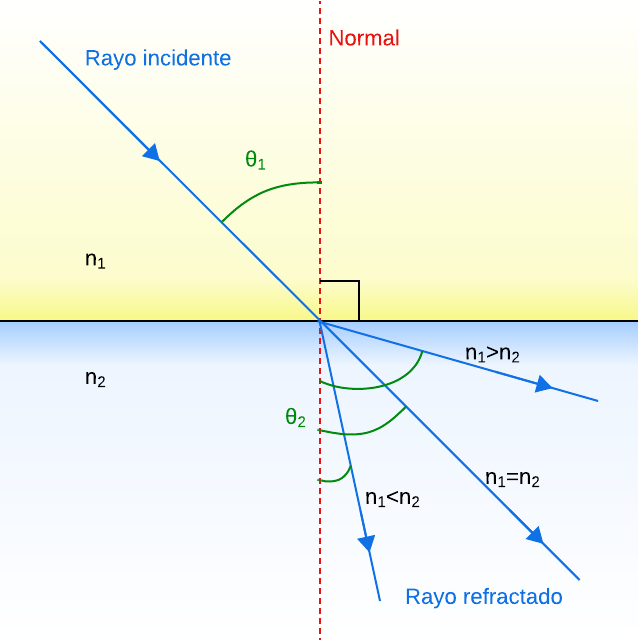
\includegraphics{imagenes/rayos_refractados.png}
  \caption{Índice de refracción y rayos refractados}
\end{figure}

\subsection{Reflexión Total Interna} \label{lbl-reftotint}
La totalidad del rayo incidente es reflejado. Ocurre cuando una onda pasa de un medio con un índice de refracción más alto a un medio con un índice de refracción más bajo, con un ángulo mayor que el \textbf{ángulo crítico}.

\begin{figure}[H]
  \centering
  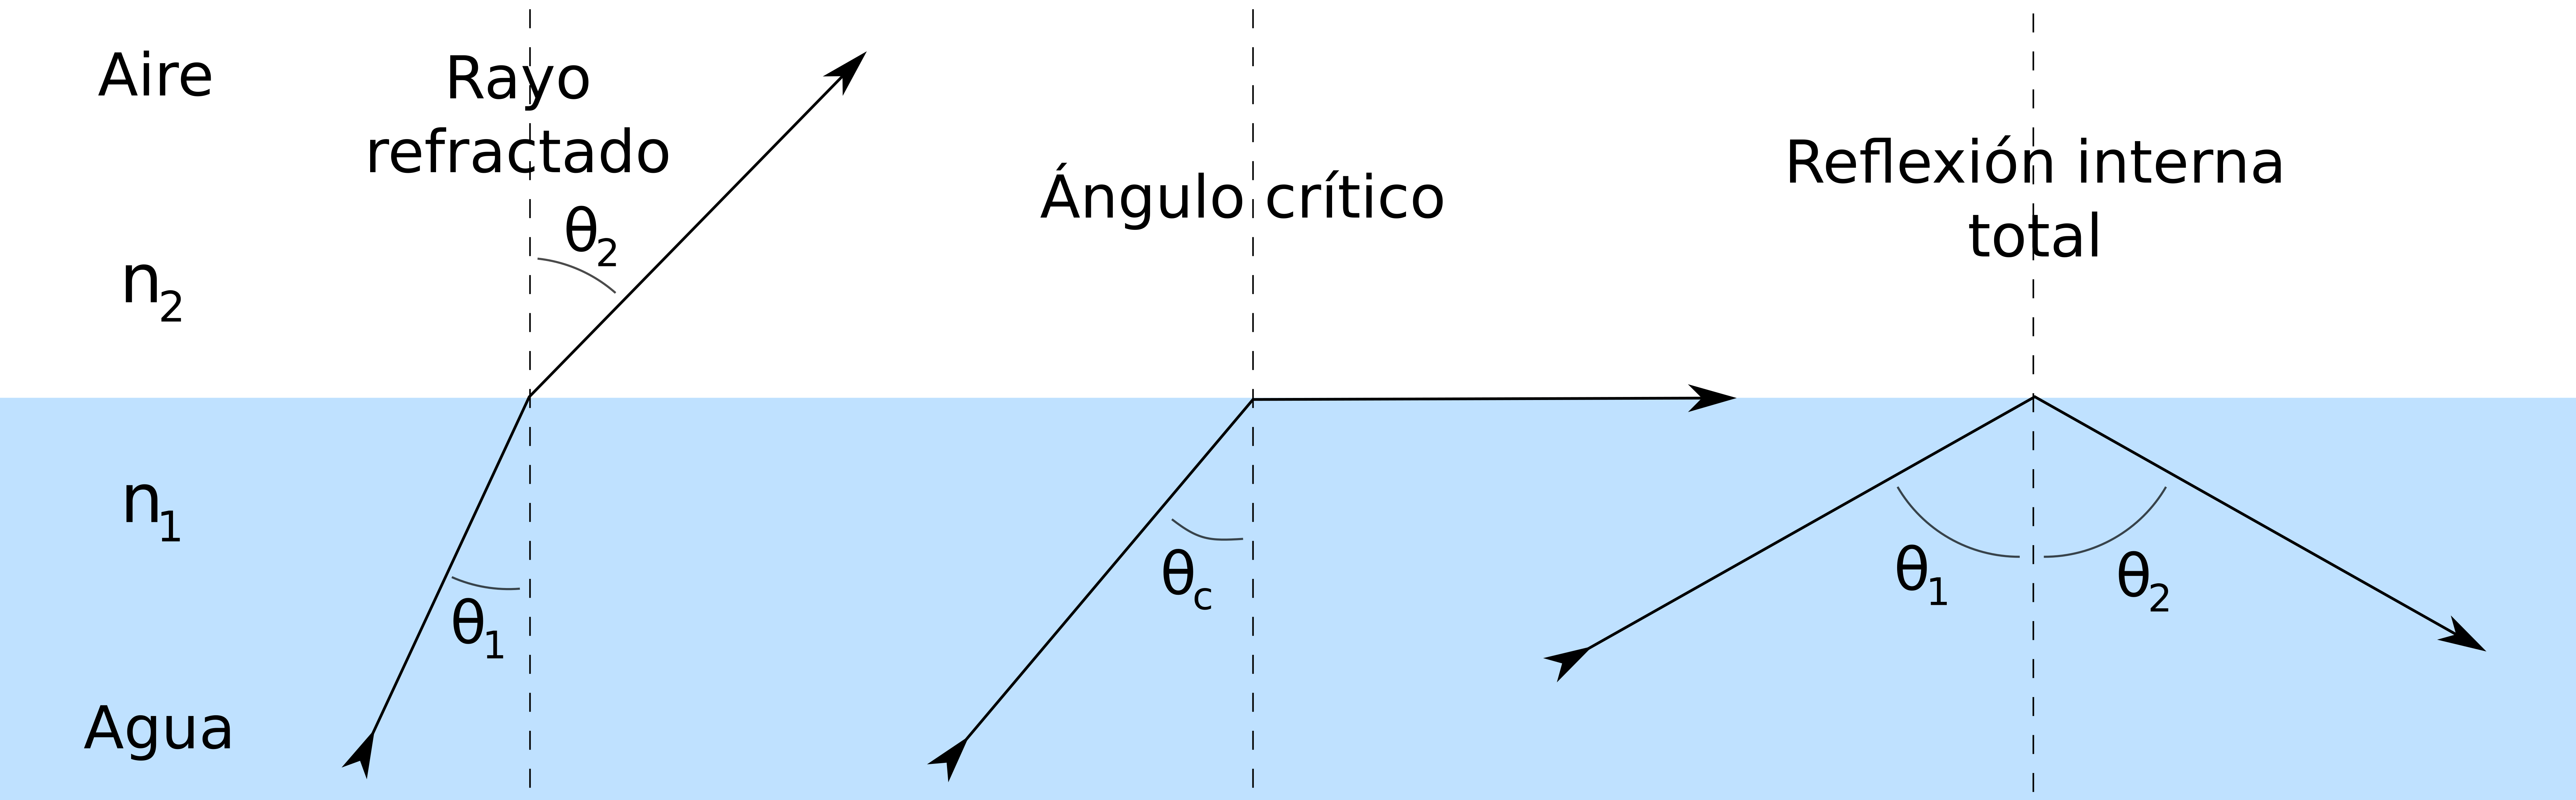
\includegraphics[scale=0.2]{imagenes/reflexion_total_interna.png}
  \caption{Reflexión total interna\cite{wikireftotint}}
\end{figure}

El ángulo crítico $(\theta_c)$ se obtiene de una variación de la ley de Snell, ecuación \ref{equleysnell}, en la cual el ángulo de refracción es de 90 grados $(\sin(90)=1)$. Donde $n_1$ y $n_2$ son los índices de refracción de los medios con $n_2 < n_1$. Se despeja el ángulo de incidencia de la siguiente forma:

\begin{listequbox}
  {\theta_c=\arcsin\left(\dfrac{n_2}{n_1}\right)}{equangcrit}{Ángulo crítico}
\end{listequbox}

% Difraccion
\section{Difracción}
Ocurre cuando una onda se encuentra con un obstáculo o abertura y se desvía, propagándose en diferentes direcciones. Puede producirse de distinas formas dependiendo del tamaño del obstáculo y la longitud de onda de la onda. Puede ocurrir alrededor o a través de un obstáculo o abertura. En este proceso se crean zonas en donde las onda no llegan o se cancelan mediante interfernecia \textbf{destructiva}.

\begin{figure}[H]
  \centering
  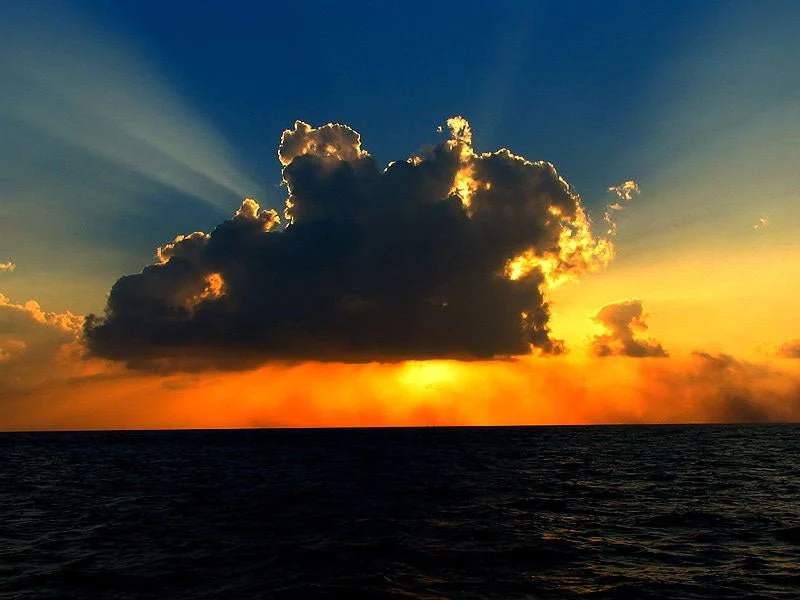
\includegraphics[scale=0.3]{imagenes/difraccion_nube.png}
  \caption{Difracción en las nubes\cite{rnbsymdfr}}
\end{figure}

Una forma simple de ver la difracción de ondas es colocar los dedos de una mano en frente de una fuente de luz y cerrarlos lentamente observando la luz pasar a través de ellos. A medida que los dedos se acercan unos a otros la luz forma patrones de lineas entre los dedos. Otra situación de esto es la luz difractada por las nubes. Esas lineas son patrones de difracción\cite{sncdfrlight}.

\subsection{Difracción alrededor de un obstáculo}
\begin{figure}[H]
  \centering
  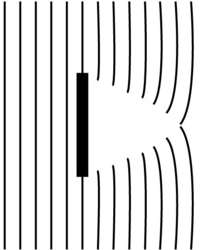
\includegraphics[scale=0.5]{imagenes/difraccion_alrededor.png}
  \caption{Difracción alrededor de un obstáculo\cite{texasdiffraction}}
\end{figure}

\subsection{Difracción a través de una abertura}
Es muy importante considerar la longitud de onda de la onda. Si el tamaño de la abertura es muy superior a la longitud de onda, la onda pasa sin ningún problema. Mientras el tamaño de la abertura se acerca a la longitud de onda la difracción se vuelve más marcada, hasta el punto donde ambos valores son muy parecidos y la curvatura de la onda difractada tiende a ser uniforme. Cuando ambos valores son iguales ocurre una difracción verdadera o completa.

\begin{figure}[H]
  \centering
  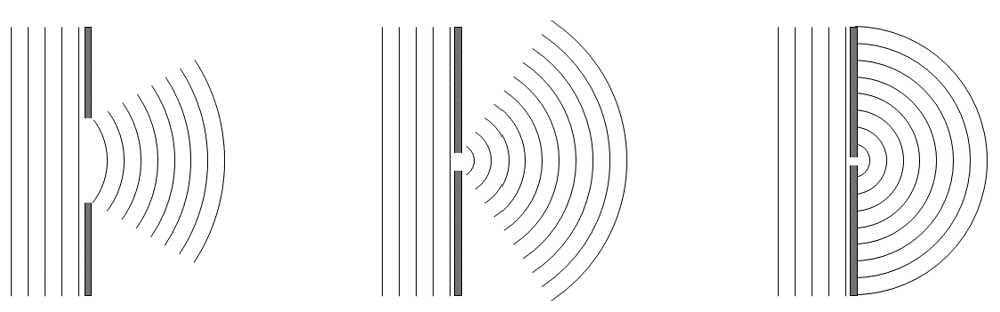
\includegraphics{imagenes/difraccion_atraves.png}
  \caption{Difracción a través de una abertura\cite{xmpdiffraction}}
\end{figure}

% Absorcion
\section{Absorción}
Proceso por el cual un medio absorbe energía de una onda que lo atraviesa, reduciendo su amplitud y eventualmente su intensidad. Ocurre cuando la energía de la onda se transforma en otra forma de energía, generalmente calor, dentro del material.

Esto se puede observar en el espectro de absorción de los hojas. La clorofila no absorbe toda la luz solar uniformemente. Las moléulas de clorofila preferentemente absorben la luz roja (con picos de aborción de $600-700 nm$ del \EspectroElectromagnetico) y azul (con picos de aborción de $400-500 nm$) para usar en la fotosíntesis, pero mucho menos en la luz verde (picos de absorción de $500-600 nm$) es absorbida y por tanto una gran cantidad es reflejada\cite{doncontrolhojas}.

\begin{figure}[H]
  \centering
  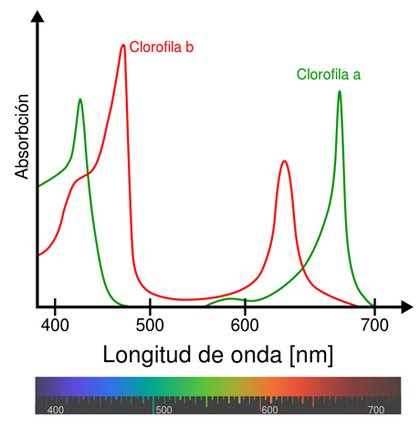
\includegraphics[scale=0.6]{imagenes/absorcion_hojas.png}
  \caption{Espectro de absorción de las hojas\cite{doncontrolhojas}}
\end{figure}

